% !TEX program = xelatex
\documentclass[11pt]{beamer}
\usetheme{Madrid}
\usecolortheme{crane}
\usepackage{graphicx}
\usepackage{booktabs}
\usepackage{amsmath,amssymb}
\usepackage{tikz}
\usetikzlibrary{shapes, arrows.meta, positioning, calc}
\usepackage{algorithm}
\usepackage{algorithmic}

\title{Transfer Learning \& Self-Supervised Learning}
\subtitle{Lecture 14 — CS F464: Introduction to Machine Learning}
\author{Shivam Sharma}
\date{Semester 2024-25 (Spring)}

\begin{document}
\maketitle

% Slide 1-2: Title + Outline
\begin{frame}{Outline}
    \tableofcontents
\end{frame}

% =====================================================
\section{Transfer Learning}
% =====================================================

% Slide 3
\begin{frame}{Motivation: Why Transfer Learning?}
    \begin{itemize}
        \item Training deep networks from scratch requires:
        \begin{itemize}
            \item Large labeled datasets (millions of samples)
            \item Significant computational resources (GPU-hours)
            \item Careful hyperparameter tuning
        \end{itemize}
        \item In practice, labeled data is scarce and expensive
        \item \textbf{Key insight}: Knowledge gained from one task can help solve another
        \item Analogy: A person who knows to ride a bicycle can learn to ride a motorcycle faster
    \end{itemize}
    \vfill
    \begin{block}{Transfer Learning}
        Using knowledge (features, weights, representations) learned from a \textbf{source task} to improve learning on a different \textbf{target task}.
    \end{block}
\end{frame}

% Slide 4
\begin{frame}{Problem Setting}
    \begin{columns}
        \column{0.5\textwidth}
        \textbf{Source Domain} $\mathcal{D}_S = \{\mathcal{X}_S, P(X_S)\}$
        \begin{itemize}
            \item Source task $\mathcal{T}_S = \{Y_S, f_S(\cdot)\}$
            \item Abundant labeled data
            \item e.g., ImageNet classification
        \end{itemize}
        \vspace{1em}
        \textbf{Target Domain} $\mathcal{D}_T = \{\mathcal{X}_T, P(X_T)\}$
        \begin{itemize}
            \item Target task $\mathcal{T}_T = \{Y_T, f_T(\cdot)\}$
            \item Limited labeled data
            \item e.g., Medical image classification
        \end{itemize}
        \column{0.5\textwidth}
        \centering
        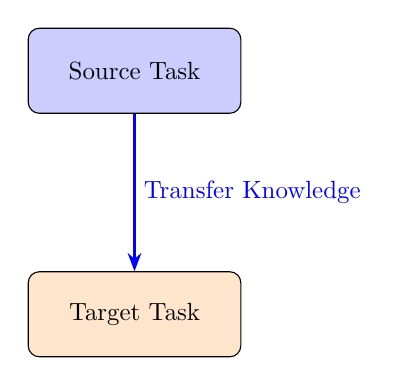
\begin{tikzpicture}[scale=0.9, every node/.style={scale=0.9}]
            \node[draw, rounded corners, fill=blue!20, minimum width=3cm, minimum height=1.2cm] (src) {Source Task};
            \node[draw, rounded corners, fill=orange!20, minimum width=3cm, minimum height=1.2cm, below=2cm of src] (tgt) {Target Task};
            \draw[-{Stealth}, thick, blue] (src) -- node[right] {Transfer Knowledge} (tgt);
        \end{tikzpicture}
    \end{columns}
\end{frame}

% Slide 5
\begin{frame}{Types of Transfer Learning}
    \begin{enumerate}
        \item \textbf{Inductive Transfer Learning}
        \begin{itemize}
            \item Source and target \emph{tasks} are different: $\mathcal{T}_S \neq \mathcal{T}_T$
            \item Domains may be same or different
            \item Most common setting in practice
            \item Some labeled target data is available
        \end{itemize}
        \item \textbf{Transductive Transfer Learning}
        \begin{itemize}
            \item Tasks are same: $\mathcal{T}_S = \mathcal{T}_T$
            \item But domains differ: $\mathcal{D}_S \neq \mathcal{D}_T$
            \item e.g., Domain adaptation (sentiment analysis: books $\to$ DVDs)
        \end{itemize}
        \item \textbf{Unsupervised Transfer Learning}
        \begin{itemize}
            \item Target task is unsupervised
            \item e.g., Clustering, anomaly detection
        \end{itemize}
    \end{enumerate}
\end{frame}

% Slide 6
\begin{frame}{Transfer Learning Strategies}
    \centering
    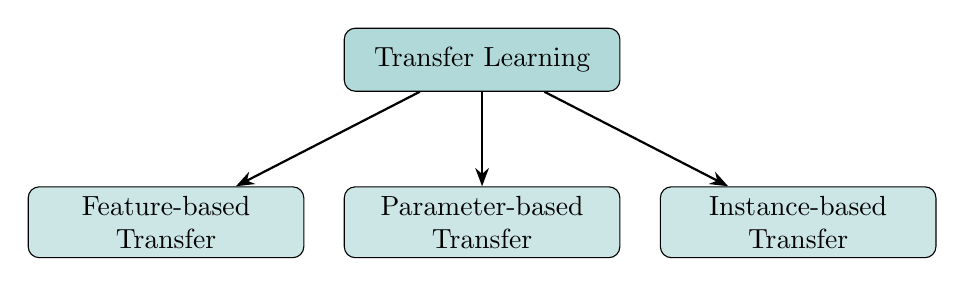
\begin{tikzpicture}[
        box/.style={draw, rounded corners, fill=teal!20, minimum width=3.5cm, minimum height=0.8cm, align=center},
        arr/.style={-{Stealth}, thick}
    ]
        \node[box, fill=teal!30] (tl) {Transfer Learning};
        \node[box, below left=1.2cm and 0.5cm of tl] (ft) {Feature-based\\Transfer};
        \node[box, below=1.2cm of tl] (param) {Parameter-based\\Transfer};
        \node[box, below right=1.2cm and 0.5cm of tl] (inst) {Instance-based\\Transfer};
        \draw[arr] (tl) -- (ft);
        \draw[arr] (tl) -- (param);
        \draw[arr] (tl) -- (inst);
    \end{tikzpicture}
    \vfill
    \begin{itemize}
        \item \textbf{Feature-based}: Use features learned from source as representation
        \item \textbf{Parameter-based}: Share model parameters/weights
        \item \textbf{Instance-based}: Re-weight source instances for target
    \end{itemize}
\end{frame}

% Slide 7-9: Feature-based Transfer
\begin{frame}{Feature-Based Transfer Learning}
    \begin{itemize}
        \item Learn a common feature representation from source domain
        \item Use these features for the target task
    \end{itemize}
    \vspace{0.5em}
    \textbf{Approach}: Train a feature extractor $\phi(\cdot)$ on source task
    \begin{itemize}
        \item \textbf{Asymmetric}: Learn features to make target data easy to classify
            \begin{itemize}
                \item TCA (Transfer Component Analysis)
                \item Metric learning approaches
            \end{itemize}
        \item \textbf{Symmetric}: Learn features that make source and target distributions similar
            \begin{itemize}
                \item Minimize Maximum Mean Discrepancy (MMD)
                \item Domain-adversarial approaches
            \end{itemize}
    \end{itemize}
\end{frame}

% Slide 10-12: Parameter-based Transfer
\begin{frame}{Parameter-Based Transfer (Pre-training \& Fine-tuning)}
    \begin{columns}
        \column{0.55\textwidth}
        \textbf{Pre-training Phase}:
        \begin{itemize}
            \item Train a model on the source task with large dataset
            \item Learn general feature representations
            \item e.g., Train ResNet on ImageNet (1000 classes)
        \end{itemize}
        \vspace{0.5em}
        \textbf{Fine-tuning Phase}:
        \begin{itemize}
            \item Copy pre-trained weights to target model
            \item Replace the final classification layer
            \item Continue training on target (small) dataset
            \item Optionally freeze early layers
        \end{itemize}
        \column{0.45\textwidth}
        \centering
        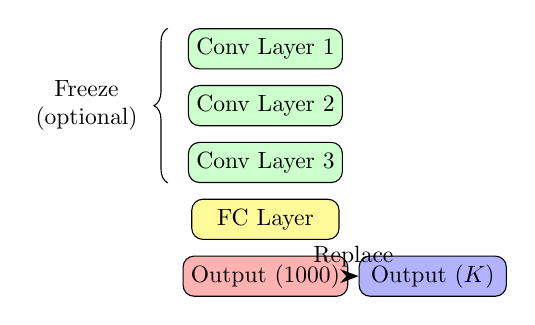
\begin{tikzpicture}[
            layer/.style={draw, minimum width=2.2cm, minimum height=0.6cm, rounded corners},
            scale=0.85, every node/.style={scale=0.85}
        ]
            \node[layer, fill=green!20] (l1) {Conv Layer 1};
            \node[layer, fill=green!20, below=0.2cm of l1] (l2) {Conv Layer 2};
            \node[layer, fill=green!20, below=0.2cm of l2] (l3) {Conv Layer 3};
            \node[layer, fill=yellow!40, below=0.2cm of l3] (l4) {FC Layer};
            \node[layer, fill=red!30, below=0.2cm of l4] (out) {Output (1000)};
            \node[layer, fill=blue!30, below=0.2cm of l4, xshift=2.5cm] (out2) {Output ($K$)};

            \draw[decorate, decoration={brace, mirror, amplitude=5pt}] ([xshift=-0.3cm]l1.north west) -- ([xshift=-0.3cm]l3.south west) node[midway, left=8pt, align=center] {Freeze\\(optional)};
            \draw[-{Stealth}, thick] (out.east) -- (out2.west) node[midway, above] {Replace};
        \end{tikzpicture}
    \end{columns}
\end{frame}

\begin{frame}{Practical Considerations for Fine-tuning}
    \begin{itemize}
        \item \textbf{Learning rate}: Use a smaller LR ($10\times$ to $100\times$ smaller) than pre-training
            \begin{itemize}
                \item Pre-training: $\eta = 0.1$; Fine-tuning: $\eta = 0.001$
            \end{itemize}
        \item \textbf{Discriminative learning rates}: Lower LR for earlier layers, higher for later layers
        \item \textbf{Gradual unfreezing}: Unfreeze layers one by one during training
        \item \textbf{How much target data?}
            \begin{itemize}
                \item Very little data ($<1000$): Freeze most layers, only train classifier
                \item Moderate data ($1000$-$10000$): Fine-tune some layers
                \item Large data ($>10000$): Fine-tune entire network
            \end{itemize}
    \end{itemize}
    \vfill
    \begin{alertblock}{Key Rule of Thumb}
        The more similar the source and target tasks, and the less target data you have, the more layers you should freeze.
    \end{alertblock}
\end{frame}

% Slide 13-14: Instance-based Transfer
\begin{frame}{Instance-Based Transfer Learning}
    \textbf{Idea}: Re-weight source domain instances to reduce distribution mismatch.
    \begin{itemize}
        \item Directly reuse source samples, but with adjusted importance weights
        \item Instances similar to target distribution get higher weight
    \end{itemize}
    \vspace{0.5em}
    \textbf{Kernel Mean Matching (KMM)}:
    \[
        \min_{w} \left\| \frac{1}{n_S} \sum_{i=1}^{n_S} w_i \phi(x_i^S) - \frac{1}{n_T} \sum_{j=1}^{n_T} \phi(x_j^T) \right\|^2
    \]
    subject to: $w_i \geq 0$, $\left|\frac{1}{n_S}\sum_{i=1}^{n_S} w_i - 1\right| \leq \epsilon$

    \vspace{0.3em}
    $\phi(\cdot)$ is a kernel-induced feature mapping (e.g., RBF kernel).
\end{frame}

% Slide 15-17: Multi-task Learning
\begin{frame}{Multi-Task Learning (MTL) as Transfer}
    \begin{columns}
        \column{0.5\textwidth}
        \begin{itemize}
            \item Train multiple related tasks simultaneously
            \item Shared representation helps all tasks
            \item Implicit transfer between tasks
            \item \textbf{Hard sharing}: All tasks share same hidden layers
            \item \textbf{Soft sharing}: Each task has own parameters, but regularized to be similar
        \end{itemize}
        \column{0.5\textwidth}
        \centering
        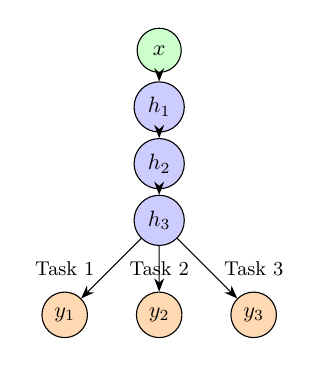
\begin{tikzpicture}[
            layer/.style={draw, circle, minimum size=0.7cm, fill=blue!20},
            output/.style={draw, circle, minimum size=0.7cm, fill=orange!30},
            scale=0.8, every node/.style={scale=0.8}
        ]
            % Shared layers
            \foreach \i in {1,2,3} {
                \node[layer] (h\i) at (0, -\i*0.9) {$h_{\i}$};
            }
            % Task-specific outputs
            \node[output] (t1) at (-1.5, -4.2) {$y_1$};
            \node[output] (t2) at (0, -4.2) {$y_2$};
            \node[output] (t3) at (1.5, -4.2) {$y_3$};
            % Input
            \node[layer, fill=green!20] (inp) at (0, 0) {$x$};
            \draw[-{Stealth}] (inp) -- (h1);
            \draw[-{Stealth}] (h1) -- (h2);
            \draw[-{Stealth}] (h2) -- (h3);
            \draw[-{Stealth}] (h3) -- (t1);
            \draw[-{Stealth}] (h3) -- (t2);
            \draw[-{Stealth}] (h3) -- (t3);
            \node[above=0.1cm of t1, font=\small] {Task 1};
            \node[above=0.1cm of t2, font=\small] {Task 2};
            \node[above=0.1cm of t3, font=\small] {Task 3};
        \end{tikzpicture}
    \end{columns}
\end{frame}

\begin{frame}{Multi-Task Learning: Objective}
    With $T$ tasks, the combined loss:
    \[
        \mathcal{L}_{\text{MTL}} = \sum_{t=1}^{T} \lambda_t \mathcal{L}_t(\theta_{\text{shared}}, \theta_t)
    \]
    \begin{itemize}
        \item $\theta_{\text{shared}}$: Shared parameters
        \item $\theta_t$: Task-specific parameters
        \item $\lambda_t$: Task weighting (can be learned)
    \end{itemize}
    \vspace{0.5em}
    \textbf{Why does MTL help?}
    \begin{itemize}
        \item \textbf{Statistical}: More data effectively seen by shared layers
        \item \textbf{Regularization}: Shared representation must work for all tasks
        \item \textbf{Eavesdropping}: Auxiliary tasks provide hints about features
    \end{itemize}
\end{frame}

% Slide 18: Progressive Neural Networks
\begin{frame}{Progressive Neural Networks}
    \begin{itemize}
        \item Addresses \emph{catastrophic forgetting} in sequential transfer
        \item Architecture grows as new tasks are added
        \item Each new column gets lateral connections from all previous columns
        \item Previous columns are frozen, so no forgetting
    \end{itemize}
    \vspace{0.5em}
    \centering
    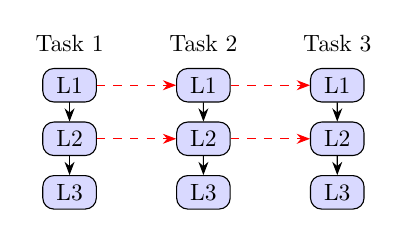
\begin{tikzpicture}[
        col/.style={draw, fill=blue!15, minimum width=0.8cm, minimum height=0.5cm, rounded corners},
        scale=0.85, every node/.style={scale=0.85}
    ]
        % Column 1
        \foreach \i in {1,2,3} { \node[col] (c1\i) at (0, -\i*0.8) {L\i}; }
        % Column 2
        \foreach \i in {1,2,3} { \node[col] (c2\i) at (2, -\i*0.8) {L\i}; }
        % Column 3
        \foreach \i in {1,2,3} { \node[col] (c3\i) at (4, -\i*0.8) {L\i}; }

        % Vertical connections
        \foreach \i [evaluate=\i as \j using int(\i+1)] in {1,2} {
            \draw[-{Stealth}] (c1\i) -- (c1\j);
            \draw[-{Stealth}] (c2\i) -- (c2\j);
            \draw[-{Stealth}] (c3\i) -- (c3\j);
        }
        % Lateral connections
        \draw[-{Stealth}, red, dashed] (c11) -- (c21);
        \draw[-{Stealth}, red, dashed] (c12) -- (c22);
        \draw[-{Stealth}, red, dashed] (c21) -- (c31);
        \draw[-{Stealth}, red, dashed] (c22) -- (c32);

        \node[above=0.1cm of c11] {Task 1};
        \node[above=0.1cm of c21] {Task 2};
        \node[above=0.1cm of c31] {Task 3};
    \end{tikzpicture}
\end{frame}

% =====================================================
\section{Domain Adaptation}
% =====================================================

% Slide 19-20
\begin{frame}{Domain Adaptation}
    \textbf{Problem}: Source and target domains have different distributions but same task.
    \begin{itemize}
        \item $\mathcal{X}_S \neq \mathcal{X}_T$ (e.g., photos vs.\ sketches)
        \item $P(X_S) \neq P(X_T)$ (different data distributions)
        \item $Y_S = Y_T$ (same label space)
    \end{itemize}
    \vfill
    \textbf{Types}:
    \begin{itemize}
        \item \textbf{Supervised DA}: Small amount of labeled target data available
        \item \textbf{Semi-supervised DA}: Only unlabeled target data
        \item \textbf{Unsupervised DA}: No labeled target data
    \end{itemize}
\end{frame}

% Slide 21-22: Domain-Adversarial Neural Networks
\begin{frame}{Domain-Adversarial Neural Networks (DANN)}
    \begin{itemize}
        \item \textbf{Goal}: Learn features that are \emph{domain-invariant} but \emph{class-discriminative}
        \item Uses a gradient reversal layer (GRL) for adversarial training
    \end{itemize}
    \centering
    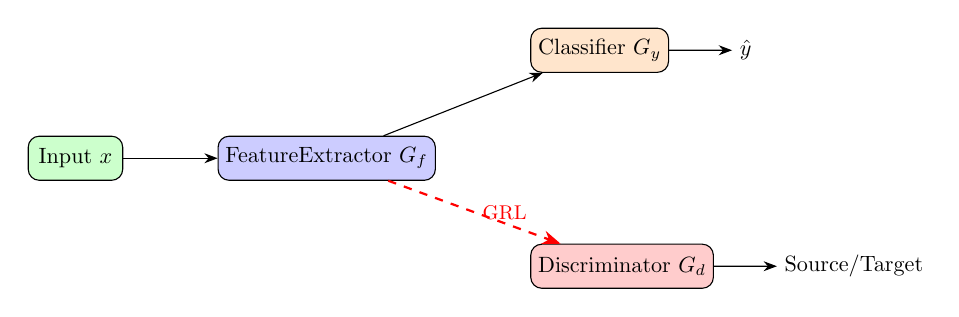
\begin{tikzpicture}[
        box/.style={draw, minimum width=1.5cm, minimum height=0.7cm, rounded corners},
        scale=0.8, every node/.style={scale=0.8}
    ]
        \node[box, fill=green!20] (input) {Input $x$};
        \node[box, fill=blue!20, right=1.2cm of input] (feat) {Feature\\Extractor $G_f$};
        \node[box, fill=orange!20, above right=0.8cm and 1.2cm of feat] (clf) {Classifier $G_y$};
        \node[box, fill=red!20, below right=0.8cm and 1.2cm of feat] (disc) {Discriminator $G_d$};
        \node[right=0.8cm of clf] (y) {$\hat{y}$};
        \node[right=0.8cm of disc] (d) {Source/Target};

        \draw[-{Stealth}] (input) -- (feat);
        \draw[-{Stealth}] (feat) -- (clf);
        \draw[-{Stealth}, dashed, red, thick] (feat) -- node[right] {\small GRL} (disc);
        \draw[-{Stealth}] (clf) -- (y);
        \draw[-{Stealth}] (disc) -- (d);
    \end{tikzpicture}
    \vspace{0.5em}

    \textbf{Objective}:
    \[
        \min_{G_f, G_y} \max_{G_d} \underbrace{\mathbb{E}[\mathcal{L}_y(G_y(G_f(x)))]}_{\text{classification loss}} - \lambda \underbrace{\mathbb{E}[\mathcal{L}_d(G_d(G_f(x)))]}_{\text{domain confusion}}
    \]
\end{frame}

% Slide 23: Maximum Mean Discrepancy
\begin{frame}{Maximum Mean Discrepancy (MMD)}
    \textbf{Idea}: Match distributions by minimizing the distance between mean embeddings in a RKHS.
    \[
        \text{MMD}^2(\mathcal{D}_S, \mathcal{D}_T) = \left\| \mathbb{E}_{x \sim P_S}[\phi(x)] - \mathbb{E}_{x \sim P_T}[\phi(x)] \right\|^2_{\mathcal{H}}
    \]
    Empirical estimate:
    \[
        \widehat{\text{MMD}}^2 = \frac{1}{n_S^2}\sum_{i,j} k(x_i^S, x_j^S) + \frac{1}{n_T^2}\sum_{i,j} k(x_i^T, x_j^T) - \frac{2}{n_S n_T}\sum_{i,j} k(x_i^S, x_j^T)
    \]
    \begin{itemize}
        \item Added as a regularization term to the loss: $\mathcal{L} = \mathcal{L}_{\text{task}} + \lambda \cdot \text{MMD}^2$
        \item Forces the feature distributions of source and target to align
    \end{itemize}
\end{frame}

% Slide 24: CORAL
\begin{frame}{CORrelation ALignment (CORAL)}
    \textbf{Idea}: Align second-order statistics (covariance) of source and target features.
    \[
        \mathcal{L}_{\text{CORAL}} = \frac{1}{4d^2} \left\| C_S - C_T \right\|_F^2
    \]
    where $C_S$ and $C_T$ are the covariance matrices of source and target features.
    \[
        C_S = \frac{1}{n_S-1}(X_S^\top X_S - \mathbf{1}^\top X_S^\top X_S \mathbf{1}/n_S)
    \]
    \begin{itemize}
        \item Simpler than MMD — only aligns covariances
        \item Computationally efficient (closed-form)
        \item Works well when distributions differ mainly in scale/rotation
    \end{itemize}
\end{frame}

% Slide 25: Deep Domain Confusion
\begin{frame}{Deep Domain Confusion (DDC)}
    \begin{itemize}
        \item Combines deep feature learning with MMD
        \item Jointly optimizes for task performance and domain alignment
    \end{itemize}
    \[
        \mathcal{L} = \mathcal{L}_{\text{classification}}(X_S, Y_S) + \lambda \cdot \text{MMD}^2(G_f(X_S), G_f(X_T))
    \]
    \begin{itemize}
        \item $G_f$: Deep feature extractor (e.g., AlexNet)
        \item Adaptation layer is chosen to minimize MMD
        \item $\lambda$ can be tuned or set via validation
    \end{itemize}
    \vfill
    \begin{block}{Summary of DA Methods}
        \centering
        \begin{tabular}{lll}
            \toprule
            Method & Mechanism & Loss \\
            \midrule
            DANN & Adversarial & Classification + Domain confusion \\
            MMD & Distribution matching & Classification + MMD \\
            CORAL & Covariance alignment & Classification + $\|C_S - C_T\|_F^2$ \\
            \bottomrule
        \end{tabular}
    \end{block}
\end{frame}

% =====================================================
\section{Self-Supervised Learning}
% =====================================================

% Slide 26-27
\begin{frame}{Self-Supervised Learning: Motivation}
    \begin{itemize}
        \item Supervised learning needs labels — expensive and limited
        \item Unlabeled data is abundant (images, text, audio)
        \item \textbf{Self-supervised learning}: Generate labels automatically from the data itself
            \begin{itemize}
                \item Design a \emph{pretext task} that forces the model to learn useful representations
                \item The learned representations are then used for downstream tasks
            \end{itemize}
    \end{itemize}
    \vfill
    \centering
    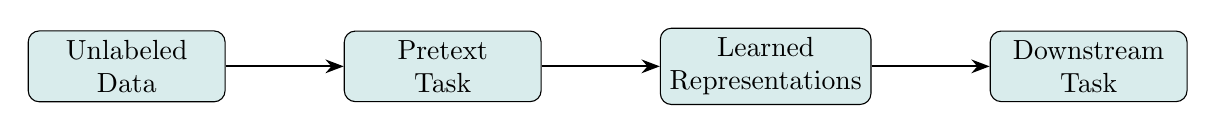
\begin{tikzpicture}[
        box/.style={draw, rounded corners, fill=teal!15, minimum width=2.5cm, minimum height=0.7cm, align=center},
        arr/.style={-{Stealth}, thick}
    ]
        \node[box] (data) {Unlabeled\\Data};
        \node[box, right=1.5cm of data] (pretask) {Pretext\\Task};
        \node[box, right=1.5cm of pretask] (repr) {Learned\\Representations};
        \node[box, right=1.5cm of repr] (downstream) {Downstream\\Task};
        \draw[arr] (data) -- (pretask);
        \draw[arr] (pretask) -- (repr);
        \draw[arr] (repr) -- (downstream);
    \end{tikzpicture}
\end{frame}

% Slide 28-29: Contrastive Learning
\begin{frame}{Contrastive Learning Framework}
    \textbf{Core idea}: Learn representations where similar pairs are close, dissimilar pairs are far apart.
    \vspace{0.5em}
    \begin{itemize}
        \item Given an \emph{anchor} sample $x$
        \item Create a \emph{positive} pair via data augmentation: $\tilde{x}_i, \tilde{x}_j$ (two views of $x$)
        \item Other samples are \emph{negatives}
    \end{itemize}
    \vfill
    \textbf{InfoNCE / NT-Xent Loss} (SimCLR):
    \[
        \ell_{i,j} = -\log \frac{\exp(\text{sim}(z_i, z_j)/\tau)}{\sum_{k=1}^{2N} \mathbb{1}_{[k \neq i]} \exp(\text{sim}(z_i, z_k)/\tau)}
    \]
    \begin{itemize}
        \item $z_i, z_j$: Projected representations of the positive pair
        \item $\text{sim}(\cdot, \cdot)$: Cosine similarity
        \item $\tau$: Temperature hyperparameter
        \item $N$: Batch size
    \end{itemize}
\end{frame}

% Slide 30-32: SimCLR
\begin{frame}{SimCLR (Chen et al., 2020)}
    \begin{enumerate}
        \item \textbf{Stochastic augmentation}: Create two views $x_i, x_j$ of same image
            \begin{itemize}
                \item Random cropping, color distortion, Gaussian blur
            \end{itemize}
        \item \textbf{Base encoder} $f(\cdot)$: Extract representations $h_i, h_j$
        \item \textbf{Projection head} $g(\cdot)$: MLP mapping to $z_i, z_j$
        \item \textbf{Contrastive loss}: Maximize agreement between $z_i, z_j$
    \end{enumerate}
    \vfill
    \centering
    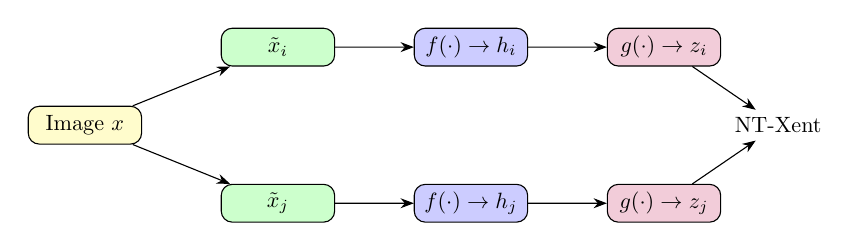
\begin{tikzpicture}[
        box/.style={draw, rounded corners, minimum width=1.8cm, minimum height=0.6cm},
        scale=0.8, every node/.style={scale=0.8}
    ]
        \node[box, fill=yellow!20] (x) {Image $x$};
        \node[box, fill=green!20, above right=0.5cm and 1cm of x] (ti) {$\tilde{x}_i$};
        \node[box, fill=green!20, below right=0.5cm and 1cm of x] (tj) {$\tilde{x}_j$};
        \node[box, fill=blue!20, right=1cm of ti] (fi) {$f(\cdot) \to h_i$};
        \node[box, fill=blue!20, right=1cm of tj] (fj) {$f(\cdot) \to h_j$};
        \node[box, fill=purple!20, right=1cm of fi] (gi) {$g(\cdot) \to z_i$};
        \node[box, fill=purple!20, right=1cm of fj] (gj) {$g(\cdot) \to z_j$};
        \node[right=0.8cm of $(gi)!0.5!(gj)$] (loss) {NT-Xent};

        \draw[-{Stealth}] (x) -- (ti);
        \draw[-{Stealth}] (x) -- (tj);
        \draw[-{Stealth}] (ti) -- (fi);
        \draw[-{Stealth}] (tj) -- (fj);
        \draw[-{Stealth}] (fi) -- (gi);
        \draw[-{Stealth}] (fj) -- (gj);
        \draw[-{Stealth}] (gi) -- (loss);
        \draw[-{Stealth}] (gj) -- (loss);
    \end{tikzpicture}
\end{frame}

\begin{frame}{SimCLR: Key Design Choices}
    \begin{itemize}
        \item \textbf{Composition of augmentations} is critical
            \begin{itemize}
                \item Random cropping + color distortion most effective
            \end{itemize}
        \item \textbf{Projection head}: MLP with one hidden layer
            \begin{itemize}
                \item $g(h) = W^{(2)} \sigma(W^{(1)} h)$
                \item Representations before projection head ($h$) are better for downstream
            \end{itemize}
        \item \textbf{Larger batch sizes} help: More negatives $\to$ better contrastive signal
            \begin{itemize}
                \item Paper uses batch sizes of 4096
            \end{itemize}
        \item \textbf{Performance}: Matches supervised pre-training on ImageNet when scaled up
    \end{itemize}
\end{frame}

% Slide 33-35: MoCo
\begin{frame}{Momentum Contrast (MoCo)}
    \textbf{Problem}: SimCLR needs very large batch sizes for enough negatives.
    \vspace{0.5em}

    \textbf{MoCo solution}: Maintain a queue of negative representations.
    \begin{itemize}
        \item \textbf{Query encoder} $f_q$: Updated by gradient descent
        \item \textbf{Key encoder} $f_k$: Updated by momentum
            \[
                \theta_k \leftarrow m \cdot \theta_k + (1-m) \cdot \theta_q \quad (m = 0.999)
            \]
        \item Positive: $z^+ = f_k(\text{aug}_2(x))$, Negative queue: $\{z^-_1, \ldots, z^-_K\}$
        \item Contrastive loss with $K$ negatives from the queue
    \end{itemize}
    \vfill
    \begin{block}{MoCo vs SimCLR}
        \begin{tabular}{lcc}
            \toprule
            & SimCLR & MoCo \\
            \midrule
            Batch size & 4096+ & 256 \\
            Negatives & In-batch & Queue ($K$=65536) \\
            Encoder & One & Two (momentum) \\
            Compute & High GPU memory & Efficient \\
            \bottomrule
        \end{tabular}
    \end{block}
\end{frame}

% Slide 36-38: BYOL / SimSiam
\begin{frame}{BYOL (Bootstrap Your Own Latent)}
    \textbf{Key insight}: Contrastive learning without negative pairs!
    \vspace{0.5em}
    \begin{itemize}
        \item \textbf{Online network}: Encoder $f_\theta$ + Projector $g_\theta$ + Predictor $q_\theta$
        \item \textbf{Target network}: Encoder $f_\xi$ + Projector $g_\xi$ (momentum-updated)
            \[
                \xi \leftarrow \tau \xi + (1-\tau)\theta
            \]
        \item \textbf{Loss}: Mean squared error between normalized predictions
            \[
                \mathcal{L} = 2 - 2 \cdot \frac{\langle q_\theta(z_\theta), z_\xi \rangle}{\|q_\theta(z_\theta)\| \cdot \|z_\xi\|}
            \]
        \item Symmetric: also compute loss with views swapped
    \end{itemize}
    \vfill
    \begin{alertblock}{Why no collapsing?}
        The predictor network $q_\theta$ and momentum update prevent representation collapse (all outputs $\to$ same vector).
    \end{alertblock}
\end{frame}

\begin{frame}{SimSiam (Simple Siamese)}
    \textbf{Further simplification}: No negative pairs, no momentum, no large batches!
    \vspace{0.5em}
    \begin{itemize}
        \item Same encoder for both views (weight sharing)
        \item Uses a predictor on one branch
        \item \textbf{Stop-gradient} on the other branch prevents collapse
    \end{itemize}
    \[
        \mathcal{L} = -\frac{\langle q_\theta(z_\theta^1), \text{sg}(z_\theta^2) \rangle}{\|q_\theta(z_\theta^1)\| \cdot \|\text{sg}(z_\theta^2)\|}
    \]
    where $\text{sg}(\cdot)$ denotes stop-gradient.
    \vfill
    \centering
    \begin{tabular}{lcccc}
        \toprule
        Method & Negatives & Momentum & Batch Size & Extra Modules \\
        \midrule
        SimCLR & Yes & No & Large & No \\
        MoCo & Yes & Yes & Small & Queue \\
        BYOL & No & Yes & Small & Predictor \\
        SimSiam & No & No & Small & Predictor \\
        \bottomrule
    \end{tabular}
\end{frame}

% Slide 39-41: Masked Autoencoders
\begin{frame}{Masked Autoencoders (MAE)}
    \textbf{Pretext task}: Mask random patches of an image, reconstruct them.
    \begin{columns}
        \column{0.55\textwidth}
        \begin{itemize}
            \item \textbf{Masking}: Randomly mask 75\% of image patches
            \item \textbf{Encoder}: ViT processes only \emph{visible} patches
            \item \textbf{Decoder}: Lightweight, takes encoded visible + mask tokens
            \item \textbf{Loss}: MSE between reconstructed and original pixel values for masked patches only
        \end{itemize}
        \column{0.45\textwidth}
        \centering
        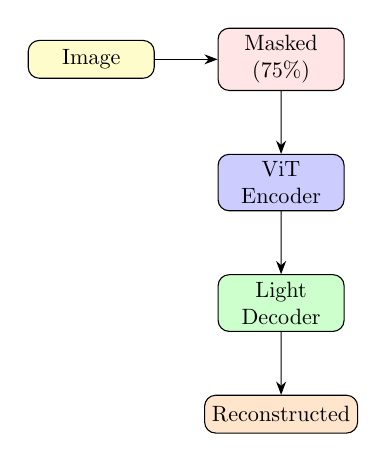
\begin{tikzpicture}[
            box/.style={draw, rounded corners, minimum width=2cm, minimum height=0.6cm, align=center},
            scale=0.8, every node/.style={scale=0.8}
        ]
            \node[box, fill=yellow!20] (img) {Image};
            \node[box, fill=red!10, right=0.8cm of img] (masked) {Masked\\(75\%)};
            \node[box, fill=blue!20, below=0.8cm of masked] (enc) {ViT\\Encoder};
            \node[box, fill=green!20, below=0.8cm of enc] (dec) {Light\\Decoder};
            \node[box, fill=orange!20, below=0.8cm of dec] (recon) {Reconstructed};

            \draw[-{Stealth}] (img) -- (masked);
            \draw[-{Stealth}] (masked) -- (enc);
            \draw[-{Stealth}] (enc) -- (dec);
            \draw[-{Stealth}] (dec) -- (recon);
        \end{tikzpicture}
    \end{columns}
\end{frame}

\begin{frame}{MAE: Why It Works}
    \begin{itemize}
        \item \textbf{High masking ratio (75\%)} forces the model to understand global context
            \begin{itemize}
                \item Can't just interpolate from neighbors
                \item Must learn high-level semantic understanding
            \end{itemize}
        \item \textbf{Asymmetric encoder-decoder}:
            \begin{itemize}
                \item Encoder only processes visible patches $\to$ very efficient
                \item Decoder is lightweight, discarded after pre-training
            \end{itemize}
        \item \textbf{Efficiency}: Encoder processes only 25\% of tokens, $\sim$3$\times$ faster training
        \item \textbf{Transfer}: Pre-trained encoder works excellently for downstream tasks
            \begin{itemize}
                \item ImageNet fine-tuning: 87.8\% top-1 (ViT-Huge)
                \item Object detection, segmentation also improved
            \end{itemize}
    \end{itemize}
\end{frame}

% Slide 42-44: NLP Self-Supervised
\begin{frame}{Self-Supervised Learning in NLP}
    \textbf{Masked Language Modeling (BERT)}:
    \begin{itemize}
        \item Mask 15\% of tokens randomly
        \item Predict the masked tokens using bidirectional context
        \item Loss: Cross-entropy over masked positions
        \[
            \mathcal{L}_{\text{MLM}} = -\mathbb{E}_{\hat{x} \sim \text{mask}(x)} \left[\log P(\hat{x} | x_{\text{masked}})\right]
        \]
    \end{itemize}
    \vspace{0.5em}
    \textbf{Next Sentence Prediction (NSP)}:
    \begin{itemize}
        \item Given sentence A and B, predict if B follows A
        \item Binary classification: [CLS] token output
    \end{itemize}
    \vfill
    \textbf{Autoregressive LM (GPT)}:
    \begin{itemize}
        \item Predict next token given previous tokens
        \item $\mathcal{L}_{\text{LM}} = -\sum_{t=1}^{T} \log P(x_t | x_{<t})$
    \end{itemize}
\end{frame}

% Slide 45: Pretext Tasks Summary
\begin{frame}{Pretext Tasks: A Taxonomy}
    \centering
    \begin{tabular}{lll}
        \toprule
        \textbf{Category} & \textbf{Method} & \textbf{Pretext Task} \\
        \midrule
        \multirow{3}{*}{Contrastive} & SimCLR & Augmentation invariance \\
         & MoCo & Queue-based contrastive \\
         & CLIP & Image-text alignment \\
        \midrule
        \multirow{2}{*}{Non-contrastive} & BYOL & Asymmetric prediction \\
         & SimSiam & Stop-gradient \\
        \midrule
        \multirow{2}{*}{Generative} & MAE & Patch reconstruction \\
         & BERT & Token prediction \\
        \midrule
        \multirow{2}{*}{Other} & RotNet & Predict rotation (0,90,180,270) \\
         & Jigsaw & Predict permutation \\
        \bottomrule
    \end{tabular}
\end{frame}

% =====================================================
\section{Advanced Topics}
% =====================================================

% Slide 46-47: LoRA
\begin{frame}{Low-Rank Adaptation (LoRA)}
    \textbf{Problem}: Fine-tuning all parameters of large models is expensive.
    \vspace{0.5em}

    \textbf{LoRA}: Freeze pre-trained weights, inject trainable low-rank matrices.
    \[
        W' = W_0 + \Delta W = W_0 + BA
    \]
    \begin{itemize}
        \item $W_0 \in \mathbb{R}^{d \times k}$: Frozen pre-trained weight
        \item $B \in \mathbb{R}^{d \times r}$, $A \in \mathbb{R}^{r \times k}$: Trainable, $r \ll \min(d,k)$
        \item Only $2 \cdot d \cdot r$ parameters per layer (vs $d \times k$ for full fine-tuning)
        \item $\alpha$ scaling: $\Delta W = \frac{\alpha}{r} BA$
    \end{itemize}
    \vfill
    \begin{block}{Advantages}
        \begin{itemize}
            \item No additional inference latency ($W' = W_0 + BA$ merged after training)
            \item Extremely parameter efficient: 0.01-0.1\% of total params
            \item Can be swapped per task (plug different LoRA adapters)
        \end{itemize}
    \end{block}
\end{frame}

\begin{frame}{LoRA: Practical Considerations}
    \textbf{Which layers to adapt?}
    \begin{itemize}
        \item Most effective: Attention matrices ($W_Q, W_V$)
        \item Can also apply to: $W_K, W_O$, FFN layers
        \item More modules $\to$ higher capacity but risk of overfitting (with small data)
    \end{itemize}
    \vspace{0.5em}
    \textbf{Rank $r$ and alpha $\alpha$}:
    \begin{itemize}
        \item Typical $r$: 4-64, $\alpha = 2r$ commonly
        \item Higher $r$ = more capacity, but diminishing returns
        \item $\alpha$ controls the magnitude of the LoRA update
    \end{itemize}
    \vspace{0.5em}
    \textbf{Hyperparameter tips}:
    \begin{itemize}
        \item Learning rate: $1e$-$4$ to $5e$-$4$ (higher than full fine-tuning)
        \item Batch size: Smaller often better for limited data
        \item Epochs: 3-10 typically
        \item Dropout: 0.05-0.1 in LoRA layers
    \end{itemize}
\end{frame}

% Slide 48: Prompt Tuning
\begin{frame}{Prompt Tuning \& Prefix Tuning}
    \textbf{Prompt Tuning} (Lester et al., 2021):
    \begin{itemize}
        \item Learn continuous ``soft prompt'' vectors prepended to input
        \item $[P_1, P_2, \ldots, P_m, x_1, x_2, \ldots, x_n]$
        \item Only the prompt vectors $P_i$ are trained
        \item Very parameter efficient: $m \times d$ parameters
    \end{itemize}
    \vfill
    \textbf{Prefix Tuning} (Li \& Liang, 2021):
    \begin{itemize}
        \item Learnable prefixes at every transformer layer (not just input)
        \item More expressive than prompt tuning
        \item Still much cheaper than full fine-tuning
    \end{itemize}
    \vfill
    \centering
    \begin{tabular}{lcc}
        \toprule
        Method & Trainable Params & Performance \\
        \midrule
        Full fine-tuning & 100\% & Highest \\
        LoRA & 0.01-0.1\% & Near full FT \\
        Prefix tuning & 0.1\% & Good \\
        Prompt tuning & 0.01\% & Moderate \\
        \bottomrule
    \end{tabular}
\end{frame}

% Slide 49-50: CLIP
\begin{frame}{CLIP (Contrastive Language-Image Pre-training)}
    \textbf{Idea}: Learn visual representations from natural language supervision.
    \begin{itemize}
        \item 400M (image, text) pairs from the internet
        \item Dual encoder: Image encoder + Text encoder
        \item Contrastive loss: Maximize cosine similarity of matching pairs
    \end{itemize}
    \[
        \mathcal{L} = -\frac{1}{N}\sum_{i=1}^{N} \log \frac{\exp(\text{sim}(I_i, T_i)/\tau)}{\sum_{j=1}^{N} \exp(\text{sim}(I_i, T_j)/\tau)}
    \]
    \vfill
    \textbf{Zero-shot classification}:
    \begin{itemize}
        \item Encode class names as text: ``A photo of a [CLASS]''
        \item Compare image embedding to all text embeddings
        \item No fine-tuning needed for new datasets!
    \end{itemize}
\end{frame}

% Slide 51-52: Knowledge Distillation
\begin{frame}{Knowledge Distillation}
    \textbf{Idea}: Transfer knowledge from a large \emph{teacher} model to a smaller \emph{student} model.
    \begin{itemize}
        \item Teacher produces \emph{soft targets} (probability distributions)
        \item Student learns to mimic these soft targets
    \end{itemize}
    \[
        \mathcal{L}_{\text{KD}} = \alpha \cdot \underbrace{\text{CE}(y, \sigma(z_s))}_{\text{hard labels}} + (1-\alpha) \cdot \underbrace{T^2 \cdot \text{KL}(\sigma(z_t/T) \| \sigma(z_s/T))}_{\text{soft labels}}
    \]
    \begin{itemize}
        \item $T$: Temperature (higher = softer distribution)
        \item $\alpha$: Weight between hard and soft targets
        \item Soft targets contain ``dark knowledge'' — inter-class relationships
    \end{itemize}
    \vfill
    \textbf{Why does it work?}
    \begin{itemize}
        \item Soft targets provide richer signal than hard labels
        \item Student learns not just \emph{what} the answer is, but \emph{why}
    \end{itemize}
\end{frame}

% Slide 53-55: Catastrophic Forgetting
\begin{frame}{Catastrophic Forgetting}
    \textbf{Problem}: Neural networks forget previously learned tasks when trained on new tasks.
    \vspace{0.5em}
    \begin{itemize}
        \item \textbf{Sequential learning}: Task A $\to$ Task B
        \item Weights optimized for Task B may overwrite Task A knowledge
    \end{itemize}
    \vfill
    \textbf{Mitigation strategies}:
    \begin{enumerate}
        \item \textbf{Elastic Weight Consolidation (EWC)}:
        \[
            \mathcal{L} = \mathcal{L}_B(\theta) + \frac{\lambda}{2}\sum_i F_i (\theta_i - \theta^*_i)^2
        \]
        Penalizes changes to important weights ($F_i$: Fisher information).
        \item \textbf{Progressive Networks}: Add new columns per task (see earlier slide)
        \item \textbf{Replay buffers}: Interleave samples from old tasks during training
    \end{enumerate}
\end{frame}

% Slide 56-57: Summary
\begin{frame}{Summary: Taxonomy of Methods}
    \centering
    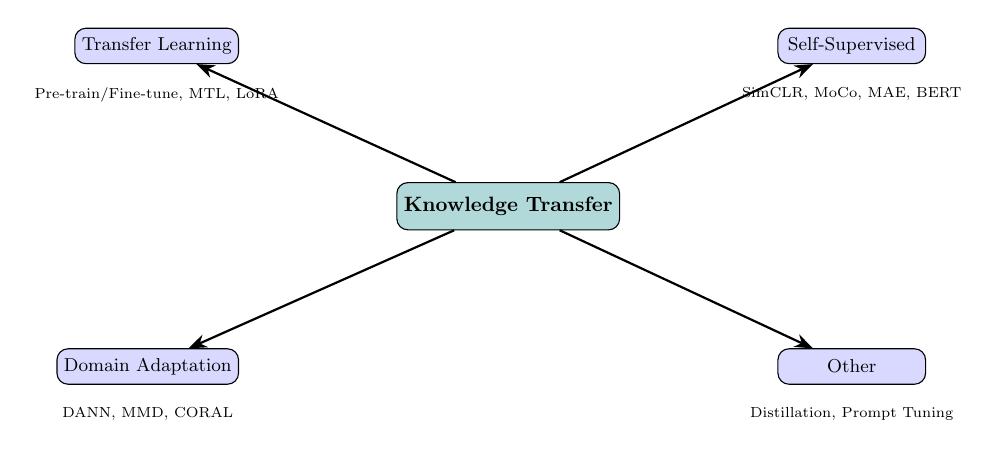
\begin{tikzpicture}[
        root/.style={draw, rounded corners, fill=teal!30, minimum width=3cm, minimum height=0.8cm, font=\bfseries},
        child1/.style={draw, rounded corners, fill=blue!15, minimum width=2.5cm, minimum height=0.6cm, font=\small},
        scale=0.75, every node/.style={scale=0.75}
    ]
        \node[root] (center) {Knowledge Transfer};
        \node[child1, above left=1.5cm and 2cm of center] (tl) {Transfer Learning};
        \node[child1, above right=1.5cm and 2cm of center] (ssl) {Self-Supervised};
        \node[child1, below left=1.5cm and 2cm of center] (da) {Domain Adaptation};
        \node[child1, below right=1.5cm and 2cm of center] (other) {Other};

        \node[font=\scriptsize, below=0.2cm of tl] {Pre-train/Fine-tune, MTL, LoRA};
        \node[font=\scriptsize, below=0.2cm of ssl] {SimCLR, MoCo, MAE, BERT};
        \node[font=\scriptsize, below=0.2cm of da] {DANN, MMD, CORAL};
        \node[font=\scriptsize, below=0.2cm of other] {Distillation, Prompt Tuning};

        \draw[-{Stealth}, thick] (center) -- (tl);
        \draw[-{Stealth}, thick] (center) -- (ssl);
        \draw[-{Stealth}, thick] (center) -- (da);
        \draw[-{Stealth}, thick] (center) -- (other);
    \end{tikzpicture}
\end{frame}

\begin{frame}{Key Takeaways}
    \begin{enumerate}
        \item \textbf{Transfer learning} is the dominant paradigm for modern ML — almost no one trains from scratch
        \item \textbf{Self-supervised learning} enables learning from unlabeled data through clever pretext tasks
        \item \textbf{Contrastive learning} (SimCLR, MoCo) learns representations by comparing augmented views
        \item \textbf{Masked modeling} (MAE, BERT) learns by predicting missing parts of input
        \item \textbf{Domain adaptation} techniques align feature distributions across domains
        \item \textbf{Parameter-efficient methods} (LoRA, prompt tuning) make fine-tuning accessible
        \item \textbf{Knowledge distillation} transfers learned knowledge to smaller models
    \end{enumerate}
    \vfill
    \begin{block}{The Big Picture}
        Pre-train on massive unlabeled data (self-supervised) $\to$ Fine-tune on downstream task (transfer learning) $\to$ Deploy efficiently (distillation/quantization).
    \end{block}
\end{frame}

% Slide 58: References
\begin{frame}{References}
    \small
    \begin{enumerate}
        \item Pan, S.~J.\ \& Yang, Q.\ (2010). A Survey on Transfer Learning. \textit{IEEE TKDE}.
        \item Chen, T.\ et al.\ (2020). A Simple Framework for Contrastive Learning of Visual Representations (SimCLR). \textit{ICML}.
        \item He, K.\ et al.\ (2020). Momentum Contrast for Unsupervised Visual Representation Learning (MoCo). \textit{CVPR}.
        \item Grill, J.-B.\ et al.\ (2020). Bootstrap Your Own Latent (BYOL). \textit{NeurIPS}.
        \item He, K.\ et al.\ (2022). Masked Autoencoders Are Scalable Vision Learners (MAE). \textit{CVPR}.
        \item Hu, E.\ et al.\ (2022). LoRA: Low-Rank Adaptation of Large Language Models. \textit{ICLR}.
        \item Radford, A.\ et al.\ (2021). Learning Transferable Visual Models From Natural Language Supervision (CLIP). \textit{ICML}.
        \item Hinton, G.\ et al.\ (2015). Distilling the Knowledge in a Neural Network. \textit{NeurIPS Workshop}.
        \item Ganin, Y.\ et al.\ (2016). Domain-Adversarial Training of Neural Networks (DANN). \textit{JMLR}.
        \item Devlin, J.\ et al.\ (2019). BERT: Pre-training of Deep Bidirectional Transformers. \textit{NAACL}.
    \end{enumerate}
\end{frame}

\end{document}
